\subsection{In situ visualization of an Inertial Confinement Fusion (ICF) simulation}

Ascent was used to visualize the results of an unprecedented 3D simulation
of two-fluid mixing in a spherical geometry to better understand hydrodynamic
instability and the transition to turbulence process that is important to
the field of inertial confinement fusion and High Energy Density (HED)
Physics. High resolution simulations of instability growth are not practical
for routine use, so high resolution simulations like this help guide the
development of sub-grid models that capture instability effects with much
less computational cost, which are used for ICF calculations.

\begin{figure}
\centering
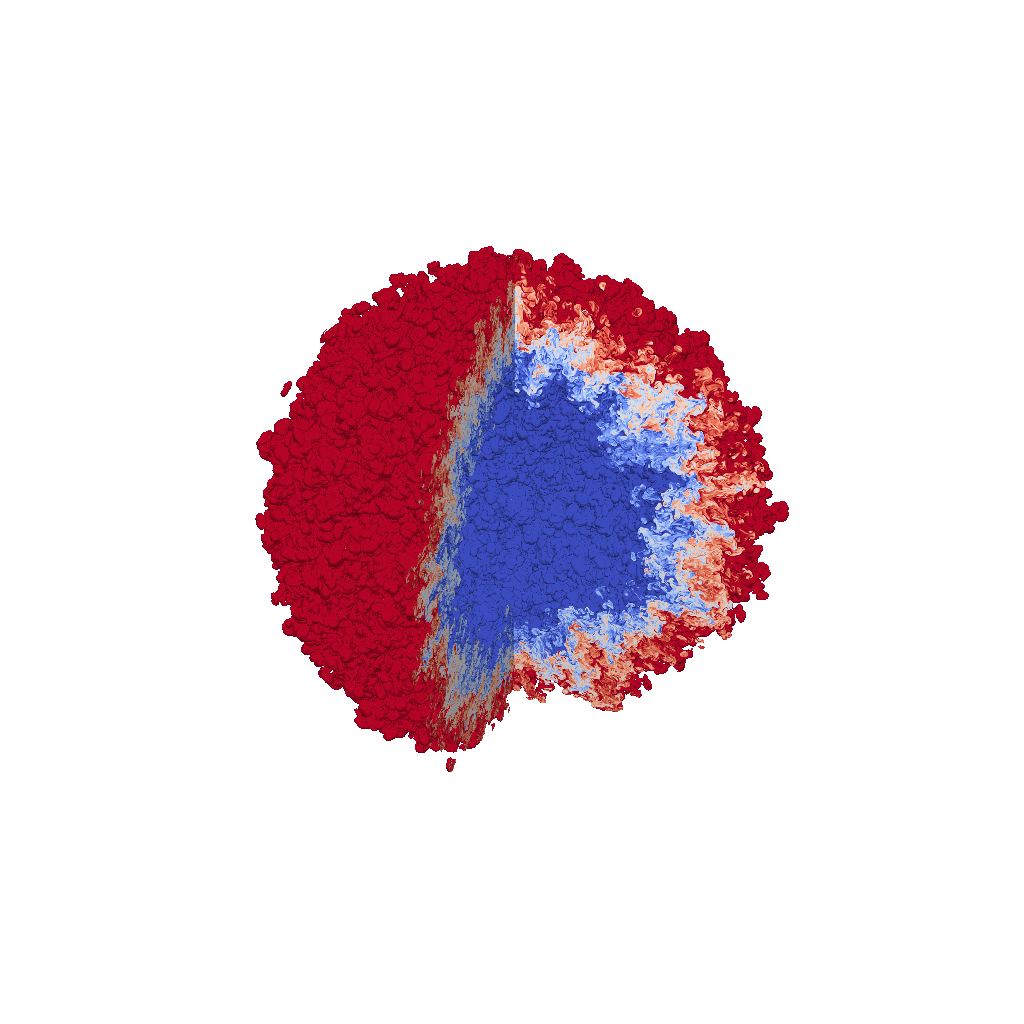
\includegraphics[trim={ 0 8cm 0 7cm},width=0.9\textwidth]{images/mixing_ball}
\caption{\label{img:icf}
This image is of an idealized Inertial Confinement
Fusion (ICF) simulation of a Rayleigh–Taylor instability
with two fluids mixing in a spherical geometry.
An isovolume filter was used to show only the mixing region of the heavy and
light fluids, and then a clip filter was added to show the internal of the sphere.
}
\end{figure}

The simulation was run on the Lawrence Livermore National Laboratory's (LLNL)
Sierra system, a 125 Petaflop peak system from IBM that has 4,320 nodes,
each with 2 IBM POWER9 processors, 4 NVIDIA Tesla V100 GPUs, 320 GiB of
fast memory (256 GiB DDR4 memory and 64 GiB HBM4), and 1.6TB of NVMe
memory. The specific simulation was a 97.8 billion element simulation
run across 16,384 GPUs on 4,096 compute nodes. The simulation application
used CUDA via RAJA to run on the GPUs. The time-varying evolution of the
mixing was visualized in situ with Ascent, also leveraging 16,384 GPUs.
The last time step was also exported by Ascent to the parallel file
system for detailed post-hoc visualization using VisIt\cite{VisIt}. The simulation
data was accessed by Ascent directly from the GPU memory, eliminating any
extra data copies.
Figure~\ref{img:icf} shows one of the many images generated in situ during
this run.

\subsection{MARBL Simulation Integration}
Ascent has been integrated and released with LLNL's MARBL~\cite{marbl} simulation code,
a new next-generation multi-physics code currently under development.
%
One of MARBL's components is a high-order finite element solver build on
MFEM~\cite{mfem}, and Ascent supports the MFEM data model.
%
In order to leverage Ascent's visualization capabilities, Ascent refines
the high-order elements to low-order(i.e., linear elements).
%
Ascent can be activated through the simulation's input deck, and in addition
to adding in situ visualization capabilities, Ascent can be used to save out
the mesh and only the fields that the user specifies.
%
Previously, MARBL only saved out full checkpoints, and only saving a subset of the
data allows users to save data for post-hoc analysis at much higher temporal resolution.

As a new code, simulation validation plays an important role, and one method
for simulation validation is comparing the results of experimental data to the
simulated experiments.
%
One such experiment is a radiation driven Kelvin-Helmholtz shear
layer experiment~\cite{hurricane2009high}.
%
The experiment captured radiographs of the instability as it was driven through
the material. Comparing experimental radiographs with radiographs created from
the simulation data is a useful simulation validation approach.
%
MARBL ran a simulation of this problem using 2304 MPI ranks for 120 hours.
%
Figure~\ref{img:radkh} shows a volume rendering and simulated radiograph
generated as a result of this simulation.
%
\begin{figure}
\centering
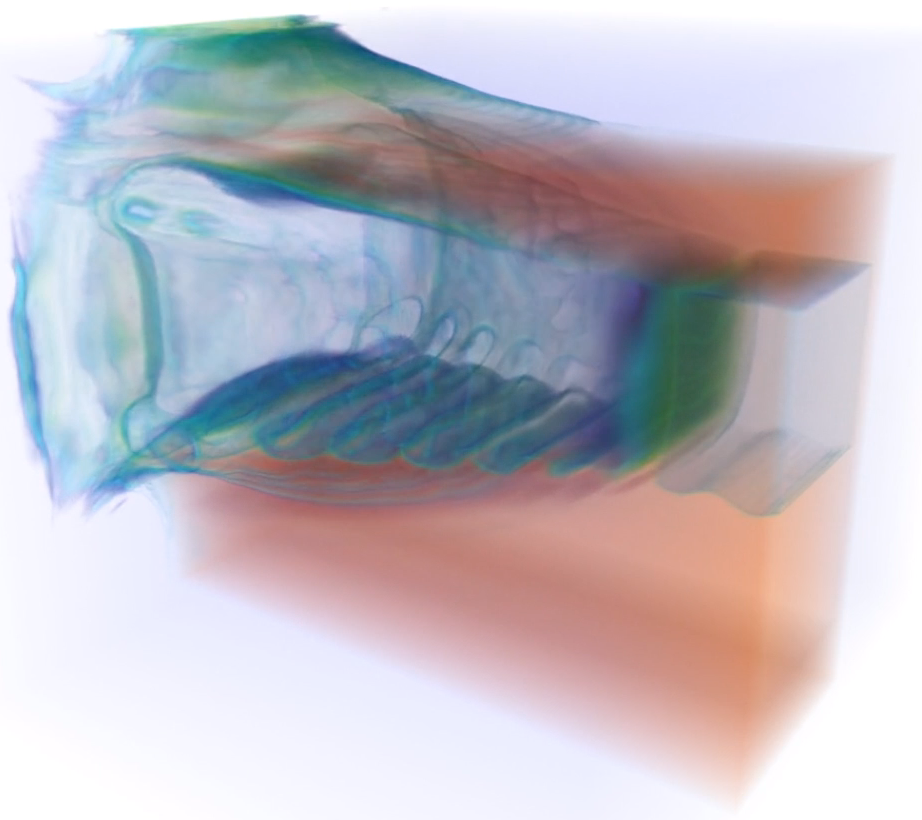
\includegraphics[width=0.4\textwidth]{images/radkh}
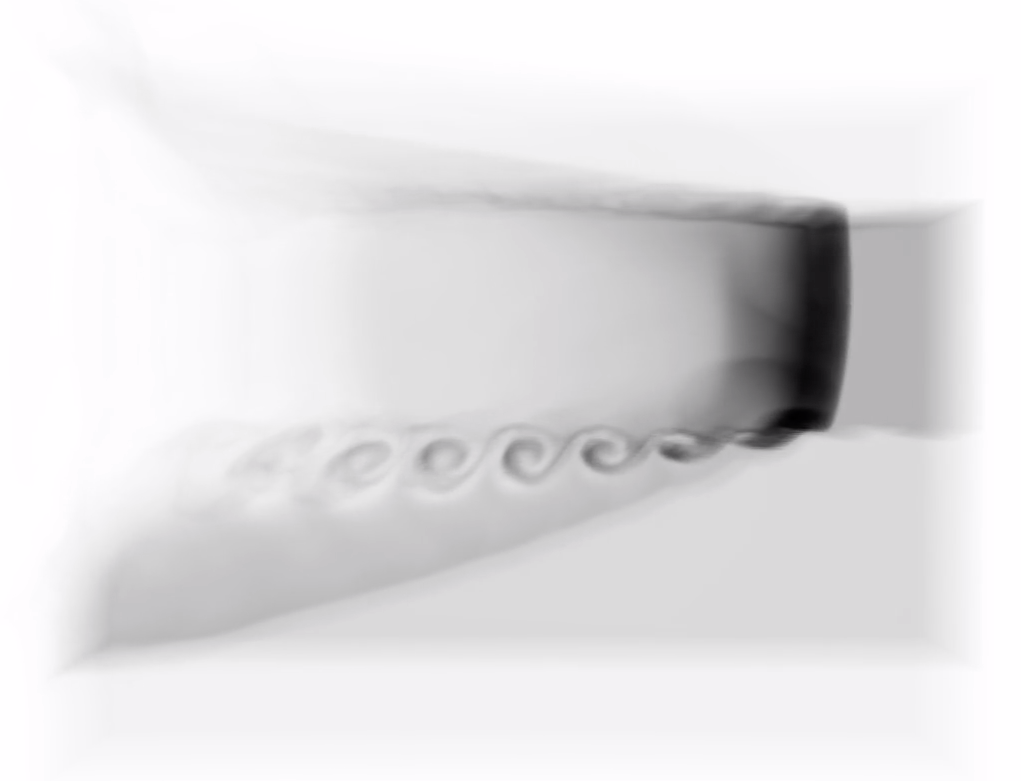
\includegraphics[width=0.4\textwidth]{images/radkh_xray}
  \caption{\label{img:radkh}A volume rendering(left) and simulated radiograph(right) created by
Ascent during a Kelvin-Helmholtz simulation.}
\end{figure}

%\subsection{Integrations}
%
%\begin{itemize}
%\item MARBL
%\item ARES
%\item AMRex: Warpx, Pele, NYX
%\item SW4
%\end{itemize}



